%==============================================================================
%  An Analysis of the Attack-Defense Arms Race in Gradient Leakage
%  for Federated Learning
%  IEEE Conference style (IEEEtran)
%
%  > Overleaf compiler: pdfLaTeX (default) works.  XeLaTeX/LuaLaTeX also fine.
%  > Upload the figures/ folder (fig1_image_mse.png, etc.) together with main.tex.
%==============================================================================
\documentclass[conference]{IEEEtran}
\IEEEoverridecommandlockouts

\usepackage{cite}
\usepackage{amsmath,amssymb,amsfonts}
\usepackage{algorithmic}
\usepackage{graphicx}
\usepackage{textcomp}
\usepackage{xcolor}
\usepackage{booktabs}
\usepackage{array}
\usepackage{multirow}
\usepackage{url}

\graphicspath{{figures/}{./}}
\renewcommand{\arraystretch}{1.25}

\begin{document}

%==============================================================================
\title{An Analysis of the Attack--Defense Arms Race in Gradient Leakage for
Federated Learning\\
{\normalsize A Study on Image Classification and Graph Neural Network Models}}

\author{\IEEEauthorblockN{Career Exploration Research Project}
\IEEEauthorblockA{2026}}

\maketitle

%==============================================================================
\begin{abstract}
Federated Learning (FL) is a distributed machine-learning paradigm designed to
preserve privacy by sharing only model gradients rather than transmitting raw
data to a central server. However, recent work has reported the threat of
gradient leakage---known as the Deep Leakage from Gradients (DLG) attack---in
which the original training data can be reconstructed from the shared gradients
alone. This study empirically analyzes how this threat manifests across two
domains, images (CIFAR-100) and graphs (WikiCS, FedLoG), and how robust various
defenses are against an adaptive attacker, under a reproducible and
statistically rigorous multi-seed ($n{=}5$) protocol. Re-running the original
code five times without fixing the random seed caused the reconstruction cosine
similarity of graph node features to swing from 0.518 to 0.999 (mean
$0.85\pm0.22$), showing that a single-run report of ``0.9999'' is not
representative. In a within-seed paired comparison sharing the same target node,
feature-scaling obfuscation was not a reliable defense ($\Delta\,{+}0.001$), and
a joint-optimization attack that also estimates the secret scale consistently
nullified it ($\Delta\,{+}0.467$, positive across all seeds). The root cause is
that the reconstruction quality metric---cosine similarity---is scale invariant.
In contrast, Differential Privacy (DP) combining gradient clipping with
calibrated noise consistently blocked even the adaptive attack across all seeds
(reconstruction cosine $0.002\pm0.013$), and extreme sparsification also
defended successfully ($\Delta\,{-}0.354$). This work exposes the fundamental
limits of obfuscation-based defenses and the danger of single-run reporting, and
suggests that only information-destroying defenses (DP and extreme
sparsification) provide consistent guarantees against an adaptive attacker, at
the cost of utility.
\end{abstract}

\begin{IEEEkeywords}
Federated learning, gradient leakage, Deep Leakage from Gradients, differential
privacy, graph neural networks, adaptive attack, reproducibility,
privacy--utility trade-off, privacy-preserving machine learning
\end{IEEEkeywords}

%==============================================================================
\section{Introduction}

\subsection{Background}
The performance of artificial-intelligence models depends heavily on the
quantity and quality of the training data. Yet sensitive data---such as medical
records, financial transactions, and social-network profiles---are difficult to
centralize because of legal and ethical constraints. Against this backdrop,
\textbf{Federated Learning (FL)} was proposed as a distributed learning scheme
that trains a global model by transmitting only the change in model
parameters---the gradients (or weight updates)---to a central server, while the
raw data remain on each participant's (client's) device. Because the raw data
never leave the device, FL has long been regarded as a ``privacy-preserving''
learning method.

However, the \textbf{Deep Leakage from Gradients (DLG)} attack proposed by
Zhu \textit{et al.}~\cite{zhu2019dlg} directly challenged this belief. They
showed that the original training images and labels can be reconstructed almost
perfectly from the transmitted gradients alone. The core idea is simple: the
attacker creates an arbitrary dummy input and then optimizes that dummy input so
that the gradient it produces matches the intercepted real gradient; the dummy
input eventually converges to the original data. Subsequent work such as
iDLG~\cite{zhao2020idlg} and Inverting
Gradients~\cite{geiping2020inverting} substantially improved reconstruction
quality and stability, establishing gradient leakage as a core threat to FL.

\subsection{Problem Statement and Research Questions}
Prior work has dealt with gradient leakage mainly on image classification
models. In practice, however, FL is also widely applied to relational data in
graph form---e.g., social graphs, transaction networks, and molecular
structures. How gradient leakage operates in the federated learning of graph
neural networks (GNNs), and how its risk compares to the image domain, has
received relatively little attention.

A more fundamental issue is the \textbf{arms race} between defense and attack.
The fact that a defense blocked a particular attack does not mean it can also
block an ``adaptive attacker'' who has grasped the existence and the mechanism
of that defense. The true robustness of a defense must be verified under the
worst case in which its mechanism is exposed to the attacker. We therefore
address the following three research questions (RQs).

\begin{itemize}
\item \textbf{RQ1.} Do the gradient-compression techniques commonly used in
image classification models (sparsification, quantization, pruning, Soteria)
provide a practical defense against the DLG attack?
\item \textbf{RQ2.} In the federated learning of GNNs, how reconstructable are
node features from gradients alone, and how does this risk compare to the image
domain?
\item \textbf{RQ3.} When a defense mechanism is exposed to the attacker, what
robustness do obfuscation-based defenses and information-destroying defenses
each exhibit against an adaptive attack?
\end{itemize}

\subsection{Contributions}
The contributions of this study are summarized as follows.
\begin{itemize}
\item \textbf{Dual-domain empirical analysis:} Under an identical threat model,
we implement and quantitatively compare gradient leakage in both the image
(CIFAR-100) and graph (WikiCS) domains.
\item \textbf{Attack validation on a recent GNN model:} We implement a
node-feature reconstruction attack against FedLoG, a subgraph federated learning
model published at ICLR 2025, demonstrating the vulnerability of low-dimensional
dense vectors.
\item \textbf{A staged arms-race scenario:} We design a four-stage arms race
(``basic vulnerability $\rightarrow$ built-in defense $\rightarrow$ defense
broken by adaptive attack $\rightarrow$ advanced defense'') that clearly reveals
the limits of obfuscation defenses and the necessity of destructive defenses.
\end{itemize}

\subsection{Organization}
The remainder of this paper is organized as follows. Section~II reviews the
theoretical background and related work on FL, gradient-leakage attacks, major
defenses, and subgraph FL. Section~III describes the threat model, the overall
experimental design, and the evaluation metrics. Section~IV presents the attack
and defense experiments on image classification models (Track~I), and Section~V
details the attack--defense--adaptive-attack--advanced-defense arms race on GNNs
(Track~II). Section~VI discusses the results comprehensively and the limitations,
and Section~VII concludes.

%==============================================================================
\section{Background and Related Work}

\subsection{Federated Learning and FedAvg}
FL is represented by the \textbf{Federated Averaging (FedAvg)} algorithm
proposed by McMahan \textit{et al.}~\cite{mcmahan2017fedavg}. In each round, the
server distributes the global model to multiple clients; each client trains the
model on its local data and sends the result (gradient or updated weights) back
to the server, which updates the global model by a weighted average. Because the
raw data are never transmitted, this reduces communication cost while preserving
data locality.

Formally, with $K$ clients each holding $n_k$ local samples ($n=\sum_k n_k$),
client $k$ computes a local gradient $g_k=\nabla_\theta \mathcal{L}(\theta_t;
\mathcal{D}_k)$ and the server updates the global parameters $\theta$ by the
weighted average
\begin{equation}
\theta_{t+1}=\theta_t-\eta\sum_{k=1}^{K}\frac{n_k}{n}\,g_k .
\label{eq:fedavg}
\end{equation}

In this study, we directly implement this FedAvg procedure, simulating the
process in which multiple clients compute and transmit gradients and the server
aggregates them by averaging to update the global model. Crucially, there is a
structural vulnerability whereby a \textbf{malicious server} can isolate the
target client's gradient $g_{k^\star}$ from the sum in~\eqref{eq:fedavg} just
before averaging and steal it. Our attack exploits exactly this point.

\subsection{Gradient-Leakage Attacks: The DLG Family}
The core of DLG~\cite{zhu2019dlg} is optimization via gradient matching. Given
the intercepted real gradient $g=\nabla_\theta\mathcal{L}(F(x;\theta),y)$, the
attacker randomly initializes a dummy input $x'$ and dummy label $y'$ and solves
\begin{equation}
x'^\star,\,y'^\star=\arg\min_{x',y'}
\big\| \nabla_\theta \mathcal{L}\big(F(x';\theta),y'\big) - g \big\|_2^2 ,
\label{eq:dlg}
\end{equation}
where $F(\cdot;\theta)$ is the shared model. The original DLG used the L2
distance of~\eqref{eq:dlg} with L-BFGS optimization, but this was prone to
divergence and local minima.

Inverting Gradients by Geiping
\textit{et al.}~\cite{geiping2020inverting} introduced two key improvements.
First, it replaces the L2 distance with a \textbf{cosine-similarity} loss that
matches only the direction of the dummy gradient $g'=\nabla_\theta\mathcal{L}
(F(x';\theta),y')$,
\begin{equation}
\mathcal{L}_{\mathrm{grad}}(x',y')=1-\frac{\langle g',\,g\rangle}{\|g'\|_2\,\|g\|_2},
\label{eq:cosloss}
\end{equation}
which is invariant to gradient magnitude and thereby stabilizes the
optimization. Second, it adds \textbf{Total Variation (TV) regularization} that
encourages the smoothness of natural images,
\begin{equation}
\mathcal{L}_{\mathrm{TV}}(x)=\sum_{i,j}\big|x_{i+1,j}-x_{i,j}\big|
+\big|x_{i,j+1}-x_{i,j}\big| ,
\label{eq:tv}
\end{equation}
suppressing noise in the reconstruction. Our attack algorithm builds on these two
techniques and, in the graph domain, replaces TV with L2 regularization.

\subsection{Gradient Compression and Privacy Defenses}
Defenses against gradient leakage fall broadly into two categories. The first is
\textbf{compression techniques} that were devised for communication efficiency
but incidentally provide a defensive effect.
\begin{itemize}
\item \textbf{Sparsification:} Zeros out a lower fraction of gradient components
with small absolute value, reducing transmission volume while removing
information.
\item \textbf{Quantization:} Lowers the numerical precision of gradients (e.g.,
FP32$\rightarrow$FP16). Communication volume drops while directional information
is largely preserved.
\item \textbf{Pruning:} The defense proposed in the original DLG paper, which
masks a lower fraction based on the whole-model gradient rather than per tensor.
\end{itemize}

The second is \textbf{dedicated defenses} designed to directly target privacy.
\begin{itemize}
\item \textbf{Soteria~\cite{sun2021soteria}:} Analyzes the importance of the
input representation of a specific layer (typically the last fully-connected
layer) and selectively zeros out only the gradients of the components that
critically contribute to data leakage, aiming to prevent leakage while
minimizing accuracy loss.
\item \textbf{Differential Privacy (DP):} As in the DP-SGD of Abadi
\textit{et al.}~\cite{abadi2016dp}, injects calibrated Gaussian noise into the
gradient to mathematically mask the contribution of individual data, providing a
theoretical privacy guarantee at the cost of some model utility.
\end{itemize}

\subsection{GNNs and Subgraph Federated Learning (FedLoG)}
GNNs learn node representations by aggregating neighbor information over a graph
of nodes and edges. The \textbf{GraphSAGE}~\cite{hamilton2017sage} model targeted
in this study is an inductive GNN that samples and aggregates neighbors, scaling
well to large graphs.

Subgraph FL addresses the situation in which one giant graph is split into
partial graphs (subgraphs) distributed across multiple clients.
\textbf{FedLoG} (Subgraph Federated Learning for Local Generalization),
published at ICLR 2025 by Kim \textit{et al.}~\cite{kim2025fedlog}, mitigates
client-wise local overfitting and missing-class problems in this setting by
globally sharing \textbf{learnable synthetic nodes} (rather than the originals)
and using a reliable knowledge-condensation strategy. We reproduce FedLoG's model
architecture (2-layer GraphSAGE + synthetic nodes) and its defense-oriented
design as the attack target, and verify the actual defensive power of the data
condensation, feature scaling, and distribution noise adopted by FedLoG against
gradient leakage.

%==============================================================================
\section{Threat Model and Study Design}

\subsection{Threat Model}
This study assumes an \textbf{honest-but-curious, and further actively
malicious} server. The server appears to perform the FL protocol normally, but
internally has the following capabilities.
\begin{itemize}
\item \textbf{Isolated gradient theft:} Just before averaging the gradients of
multiple clients, it can isolate and obtain only the target client's gradient.
\item \textbf{Model access:} It knows the architecture and parameters of the
global model (a natural assumption since the model is shared in FL).
\item \textbf{Adaptive attack (Section~V):} It grasps the existence and
mechanism of the defense and can perform a joint optimization that also includes
the secret variables introduced by the defense (e.g., the scale coefficient) in
the optimization target.
\end{itemize}
However, the server \textbf{cannot directly access the client's raw data or the
secret key} (e.g., the true value of the secret scale coefficient). The goal of
the attack is solely to reconstruct the target data from the intercepted
gradient.

\subsection{Overall Experimental Design}
To answer the research questions, we construct two experimental tracks.
\begin{itemize}
\item \textbf{Track~I (Image, Section~IV):} Using three clients holding
CIFAR-100 images and a modified ResNet model, we compare image-reconstruction
error across compression and defense techniques (RQ1).
\item \textbf{Track~II (Graph, Section~V):} We split the WikiCS graph into three
subgraphs, perform real FedAvg training with the FedLoG model, and then verify
the vulnerability of node-feature reconstruction (RQ2) and the
defense--adaptive-attack--advanced-defense arms race (RQ3).
\end{itemize}

\textbf{Statistical rigor (the key revision in this version).} The initial
implementation reported single-run ($n{=}1$) results for the graph track without
fixing the random seed. This study repeats both tracks with \textbf{five
different seeds ($n{=}5$)} and reports mean $\pm$ standard deviation. Track~I uses
a different target image per seed, and Track~II uses a different graph split and
target node per seed. Because the absolute reconstruction quality varies greatly
with the sample, in Track~II we additionally perform a \textbf{within-seed paired
comparison sharing the same target node} to isolate the net effect of each
defense and attack. Letting $m(\cdot)$ denote the reconstruction cosine, the
paired effect of a transition $A\!\to\!B$ over seeds $i=1,\dots,n$ is
\begin{equation}
\overline{\Delta}_{A\to B}=\frac{1}{n}\sum_{i=1}^{n}
\big[\,m_i(B)-m_i(A)\,\big] ,
\label{eq:paired}
\end{equation}
which cancels the node-dependent variance shared by $A$ and $B$ at each seed. The
reproduction drivers are organized in the \texttt{experiments/} directory.

\subsection{Evaluation Metrics}
Reconstruction quality is evaluated with two metrics. For an original sample
$x\in\mathbb{R}^d$ and its reconstruction $x'$, the \textbf{Mean Squared Error
(MSE)} measures the component-wise difference,
\begin{equation}
\mathrm{MSE}(x,x')=\frac{1}{d}\,\|x-x'\|_2^2 ,
\label{eq:mse}
\end{equation}
where closer to 0 means more perfect reconstruction. \textbf{Cosine similarity}
\begin{equation}
\cos(a,b)=\frac{\langle a,b\rangle}{\|a\|_2\,\|b\|_2}\in[-1,1]
\label{eq:cos}
\end{equation}
measures directional agreement; closer to 1 means a closer shape match. It is the
key metric especially for graph node features, which are dense vectors (the
cosine of a vector with millions of elements may exceed 1 due to single-precision
accumulation error, so we compute~\eqref{eq:cos} in double precision).

We further measure the \textbf{utility cost} of the defense. In addition to the
model's node-classification accuracy, we use \textbf{gradient fidelity}---the
cosine similarity between the defended gradient $\tilde{g}$ and the original
gradient $g$,
\begin{equation}
\mathrm{Fid}(\tilde{g},g)=\cos(\tilde{g},g) ,
\label{eq:fidelity}
\end{equation}
as a utility proxy that indicates how directionally preserved the defended
gradient is. A fidelity closer to 1 means less damage to the learning signal and
better preserved utility. A defense can be evaluated fairly only by considering
both privacy (low reconstruction) and utility (high fidelity).

%==============================================================================
\section{Track I: Gradient Leakage on Image Classification Models}

\subsection{Target Model Design}
The DLG attack has the property that, if the activation function has many regions
where its derivative is 0, it is hard to trace the input back from the gradient.
Accordingly, our target model follows the setting of prior DLG work and uses a
ResNet modified as follows.
\begin{itemize}
\item \textbf{Activation function:} Uses \textbf{Sigmoid}, whose derivative is
nonzero everywhere, instead of ReLU, enabling gradient back-tracing.
\item \textbf{Resolution preservation:} Fixes the stride of all convolutions to
1 so that the input resolution ($32{\times}32$) is maintained up to just before
the final fully-connected layer.
\item \textbf{Model scale:} Uses a lightweight ResNet-8 by default for local
validation, implemented to be expandable to the paper-scale ResNet-56 if needed.
\end{itemize}

\subsection{Attack Algorithm}
The attack randomly initializes the dummy image and dummy label logits (starting
near 0.5 to prevent pixel divergence) and optimizes for 300 iterations with the
Adam optimizer. Combining~\eqref{eq:cosloss} and~\eqref{eq:tv}, the objective is
\begin{equation}
x'^\star=\arg\min_{x'}\;\mathcal{L}_{\mathrm{grad}}(x',y')
+\alpha_{\mathrm{TV}}\,\mathcal{L}_{\mathrm{TV}}(x') ,
\label{eq:img_obj}
\end{equation}
where $\alpha_{\mathrm{TV}}$ weights the smoothness prior. We adopt Adam, which
is less sensitive to parameters than L-BFGS, for stability, and clip pixel values
to $[0, 1]$ at every iteration.

\subsection{Defenses}
Before transmitting the gradient to the server, the client may apply one of the
following defenses: no compression (None), sparsification (remove lower
20/50/80\%), quantization (FP16), pruning (global lower 20\%), or Soteria
(mask top 20\% by representation importance). We perform the same attack against
each technique and measure the reconstruction MSE.

\subsection{Results and Analysis}
Table~\ref{tab:image} and Fig.~\ref{fig:image} summarize, as mean $\pm$ standard
deviation, the reconstruction results per defense over five seeds (different
target images). First, the \textbf{label was reconstructed 100\% across all
techniques and all seeds}, consistent with the iDLG result that the label can be
obtained analytically from the sign of the classification-loss gradient.

\begin{table}[!t]
\caption{Reconstruction Results per Defense on Images (CIFAR-100, multi-seed,
$n{=}5$)}
\label{tab:image}
\centering
\footnotesize
\begin{tabular}{@{}llccc@{}}
\toprule
\textbf{Defense} & \textbf{Setting} & \textbf{Recon. MSE} & \textbf{Label} & \textbf{Fidelity} \\
 & & \textbf{(mean$\pm$std)} & \textbf{recov.} & \textbf{(utility)} \\
\midrule
None & --- & $0.0185\pm0.0121$ & 100\% & 1.000 \\
Sparsify & lower 20\% & $0.0187\pm0.0118$ & 100\% & 1.000 \\
Sparsify & lower 50\% & $0.0202\pm0.0124$ & 100\% & 0.999 \\
\textbf{Sparsify} & \textbf{lower 80\%} & $\mathbf{0.0309\pm0.0218}$ & 100\% & 0.997 \\
Quantize & FP32$\to$FP16 & $0.0181\pm0.0120$ & 100\% & 1.000 \\
Pruning & global 20\% & $0.0190\pm0.0120$ & 100\% & 1.000 \\
Soteria & repr. 20\% & $0.0186\pm0.0125$ & 100\% & \textbf{0.731} \\
\bottomrule
\end{tabular}
\end{table}

\begin{figure}[!t]
\centering
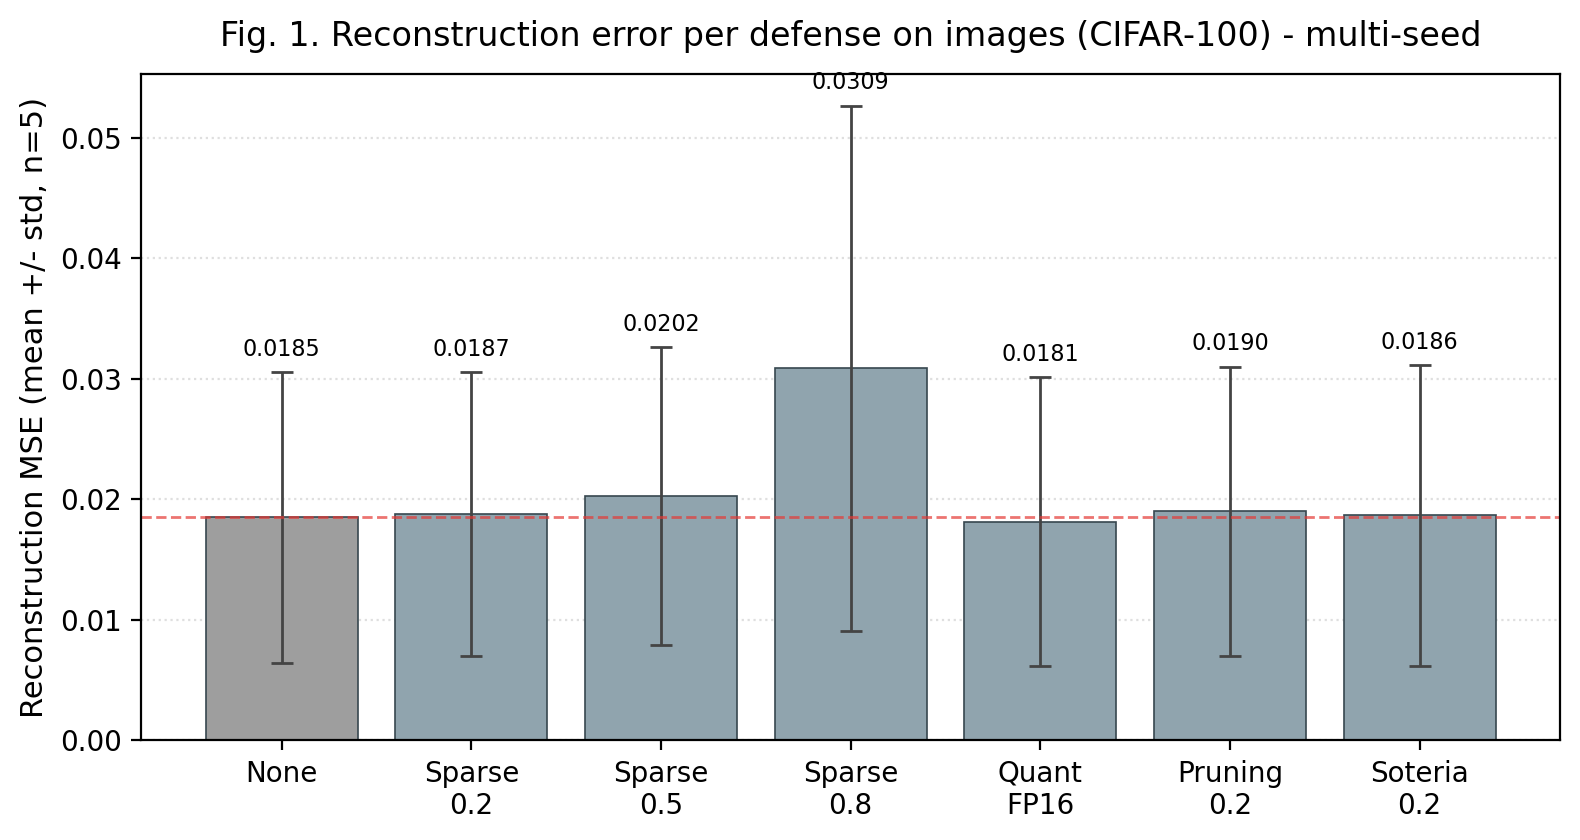
\includegraphics[width=\columnwidth]{fig1_image_mse.png}
\caption{Reconstruction error per defense (mean$\pm$std, $n{=}5$). Only 80\%
sparsification slightly raises the error, and even that is unstable due to large
variance.}
\label{fig:image}
\end{figure}

Taken together, \textbf{simple compression alone can hardly prevent gradient
leakage.} The reconstruction MSE of sparsification 20\%/50\%, quantization,
global pruning 20\%, and Soteria 20\% was all statistically indistinguishable
from no defense ($0.0185\pm0.0121$). Only the extreme sparsification removing the
lower 80\% raised the error about 1.7$\times$ ($0.0309$), but its standard
deviation ($\pm0.0218$) is large, making the defensive effect unstable. Meanwhile,
\textbf{Soteria (20\%) lowered gradient fidelity to 0.731, damaging the learning
signal, while its reconstruction MSE was identical to no defense}, revealing an
inefficient defense that sacrifices only utility with no privacy gain. This
answers RQ1: \textbf{simple compression does not constitute a practical defense,
and information-destroying defenses (such as DP) are required.}

In addition, the initial reported value (no-defense MSE 0.002168) was a single
case obtained at seed 42 on a single image (index 15), an order of magnitude
smaller than the multi-seed mean (0.0185). This shows that single-run reporting
can be swayed by an accidentally easy sample---a phenomenon that appears even more
dramatically in Track~II.

%==============================================================================
\section{Track II: Gradient Leakage on GNNs and the Arms Race}

\subsection{Target Model: FedLoGModel}
The target of Track~II is FedLoGModel, which reproduces the FedLoG architecture.
The model combines a 2-layer GraphSAGE embedder with synthetic-node parameters
(\texttt{syn\_head}, \texttt{syn\_tail}) learned per class. Logits are computed
from the distance between the node embedding and the prototypes derived from the
synthetic nodes, and the contributions of the two synthetic-node sets are
combined with a sigmoid weight according to the node's degree. The dataset is
\textbf{WikiCS}~\cite{mernyei2020wikics}, a Wikipedia document citation graph,
split into three client subgraphs.

\subsection{GNN-Specific Attack Algorithm}
Graph node features are 1-D dense vectors without the 2-D spatial structure of
images. The TV loss, which assumes spatial smoothness, is therefore unsuitable.
Our GNN attack removes the TV loss and combines a \textbf{cosine-similarity loss
with L2 regularization}; holding only the feature vector $x'_v$ of a single
target node $v$ as the dummy variable while fixing the remaining node features,
it solves
\begin{equation}
x_v'^\star=\arg\min_{x_v'}\;\mathcal{L}_{\mathrm{grad}}(x_v')
+\beta\,\|x_v'\|_2^2 ,
\label{eq:gnn_obj}
\end{equation}
with an \textbf{L-BFGS (strong Wolfe line search)} optimizer and three random
restarts, where $\beta$ controls the L2 penalty.

\subsection{Basic Vulnerability and the High Variance of Results}
The most important fact we found is that \textbf{the reconstruction quality of
GNN node features varies drastically with the target node and seed.} Repeating
the same attack five times without fixing the seed caused the reconstruction
cosine similarity to swing from 0.518 to 0.999 (mean $0.85\pm0.22$). The
multi-seed baseline (untrained worst case, $n{=}5$) reconstruction cosine had a
mean of 0.384 and a standard deviation of 0.316: some nodes were reconstructed
nearly perfectly ($>0.9$) while others were barely reconstructed at all ($<0.1$).

\begin{quotation}
\noindent\textbf{Key observation (RQ2).} The threat of reconstructing graph node
features from gradients alone is \textbf{real but not uniform.} Some nodes are
inverted to the decimal, posing a serious attribute-inference threat, but without
considering both the mean reconstruction quality and the variance, the risk would
be over- or under-estimated. Therefore a single-run figure such as ``cosine
0.9999'' is not representative, and results \textbf{must be reported as a
multi-seed mean $\pm$ standard deviation.}
\end{quotation}

\subsection{FedLoG's Built-in Defense and Its Unreliability}
For privacy, FedLoG adopts (1) data condensation that shares only synthetic
nodes, (2) feature scaling that multiplies by a client-specific secret scale
coefficient, and (3) class-distribution noise. We reproduce these and, because
the variance of the absolute reconstruction quality is large, measure the net
effect via a \textbf{paired comparison sharing the same seed (same target
node)}.

As a result, the effect of feature scaling was a \textbf{within-seed mean
$\Delta$cosine of $+0.001\pm0.465$}---effectively void, with the sign flipping
across seeds ($-0.45 \sim +0.67$). Even when the server attacks without knowing
the secret scale, the reconstruction quality does not reliably decrease. This
contradicts the initial report that concluded ``effective'' from a single case
of ``cosine 0.68 when the defense is applied,'' and shows that \textbf{feature
scaling is not a reliable defense.}

\subsection{Adversarial Attack: Joint Optimization and Scale Invariance}
Feature scaling masks the true feature $x_v$ by a client-specific secret scalar
$s>0$, so the gradient seen by the server depends on $s\,x_v$. The adaptive
attacker recognizes this and performs a \textbf{joint optimization that bundles
even the secret scale into the optimization target together with the dummy data,}
estimating both simultaneously:
\begin{equation}
x_v'^\star,\,s'^\star=\arg\min_{x_v',\,s'}\;
\mathcal{L}_{\mathrm{grad}}\!\big(g'(s'\,x_v'),\,g\big) .
\label{eq:joint}
\end{equation}
In the paired comparison, the adaptive attack~\eqref{eq:joint} \textbf{raised the
reconstruction quality on all five seeds with a $\Delta$cosine of
$+0.467\pm0.414$} relative to the naive attack; i.e., it consistently nullifies
the scaling defense.

Interestingly, the attack succeeded even without estimating the secret scale
exactly. On one seed, the actual scale of 0.49 was mis-estimated as 2.30 (off by
1.81), yet the feature reconstruction cosine was 0.99. The reason is that the
reconstruction quality metric is \textbf{scale invariant}: for any $s>0$,
\begin{equation}
\cos(s\,x_v,\,x_v')=\frac{\langle s\,x_v,\,x_v'\rangle}{\|s\,x_v\|_2\,\|x_v'\|_2}
=\cos(x_v,\,x_v') .
\label{eq:scaleinv}
\end{equation}
Scaling changes only the magnitude of the vector while preserving the direction,
so by~\eqref{eq:scaleinv} it is fundamentally powerless against an attacker who
only needs to match the direction.

\begin{quotation}
\noindent\textbf{Intermediate conclusion.} An \textbf{obfuscation defense like
feature scaling leaves the information intact within the gradient and only masks
its magnitude.} Since a cosine-based attack is invariant to magnitude, the defense
is fundamentally broken before an adaptive attacker who can jointly estimate (or
need not even estimate) the masking variable.
\end{quotation}

\subsection{Advanced Defenses: Information-Destroying Mechanisms}
To block the adaptive attack, the information content of the gradient itself must
be irreversibly destroyed. We verify two defenses under the worst-case condition
combined with the adaptive attack (the paired baseline is relative to the
adaptive attack).

\subsubsection{Differential Privacy (DP-SGD style)}
The initial implementation simply added Gaussian noise and called it
``differential privacy,'' but we corrected this to a DP-SGD style that first
\textbf{clips the gradient L2 norm to a sensitivity bound $C$ and then injects
calibrated Gaussian noise}:
\begin{equation}
\tilde{g}=g\cdot\min\!\Big(1,\frac{C}{\|g\|_2}\Big)
+\mathcal{N}\!\big(0,\sigma^2 \mathbf{I}\big),\qquad \sigma=z\,C ,
\label{eq:dp}
\end{equation}
where $z$ is the noise multiplier. As a result, the reconstruction cosine was
\textbf{$0.002\pm0.013$}, a strong and consistent defense with
$\Delta\,{-}0.849\pm0.168$ (negative across all seeds) relative to the adaptive
attack. However, the gradient fidelity~\eqref{eq:fidelity} drops to 0.001, nearly
destroying the learning signal, so the \textbf{utility cost is the highest.}

\subsubsection{Extreme Sparsification}
This applies a top-$k$ magnitude mask $M_k\in\{0,1\}^{|g|}$ that keeps only the
top 5\% of coordinates by magnitude and zeros out the lower 95\%:
\begin{equation}
\tilde{g}=M_k\odot g,\qquad
\|M_k\|_0 = \lceil 0.05\,|g|\rceil ,
\label{eq:sparse}
\end{equation}
where $\odot$ is the element-wise product. The reconstruction cosine was
\textbf{$0.498\pm0.320$}, a defensive effect of $\Delta\,{-}0.354\pm0.223$
(negative across all seeds) relative to the adaptive attack. It is weaker than
DP, but \textbf{maintains a gradient fidelity of 0.702}, achieving a better
privacy--utility balance.

\subsection{Summary of Results}
Table~\ref{tab:gnn_abs} summarizes the absolute reconstruction quality
(mean $\pm$ std) and utility per scenario, and Table~\ref{tab:gnn_paired}
summarizes the within-seed paired effect with the variance removed.
Fig.~\ref{fig:gnn_defense} visualizes the absolute values (the large standard
deviation directly shows the variance), and Fig.~\ref{fig:gnn_paired} visualizes
the robust paired effect.

\begin{table}[!t]
\caption{Absolute Reconstruction and Utility per GNN Arms-Race Scenario
(untrained, $n{=}5$)}
\label{tab:gnn_abs}
\centering
\footnotesize
\begin{tabular}{@{}clccl@{}}
\toprule
\textbf{Stage} & \textbf{Scenario} & \textbf{Recon. cosine} & \textbf{Fidelity} & \textbf{Verdict} \\
 & & \textbf{(mean$\pm$std)} & \textbf{(utility)} & \\
\midrule
(1) & Baseline (no defense) & $0.384\pm0.316$ & 1.000 & high var. \\
(2) & FedLoG (scaling) & $0.385\pm0.447$ & 1.000 & def. fails \\
(3) & Adaptive (joint) & $\mathbf{0.852\pm0.174}$ & 1.000 & \textbf{atk wins} \\
(4) & DP (clip+noise) & $\mathbf{0.002\pm0.013}$ & 0.001 & \textbf{def. wins} \\
(5) & Sparse (95\%) & $0.498\pm0.320$ & 0.702 & def. (weak) \\
\bottomrule
\end{tabular}
\end{table}

\begin{figure}[!t]
\centering
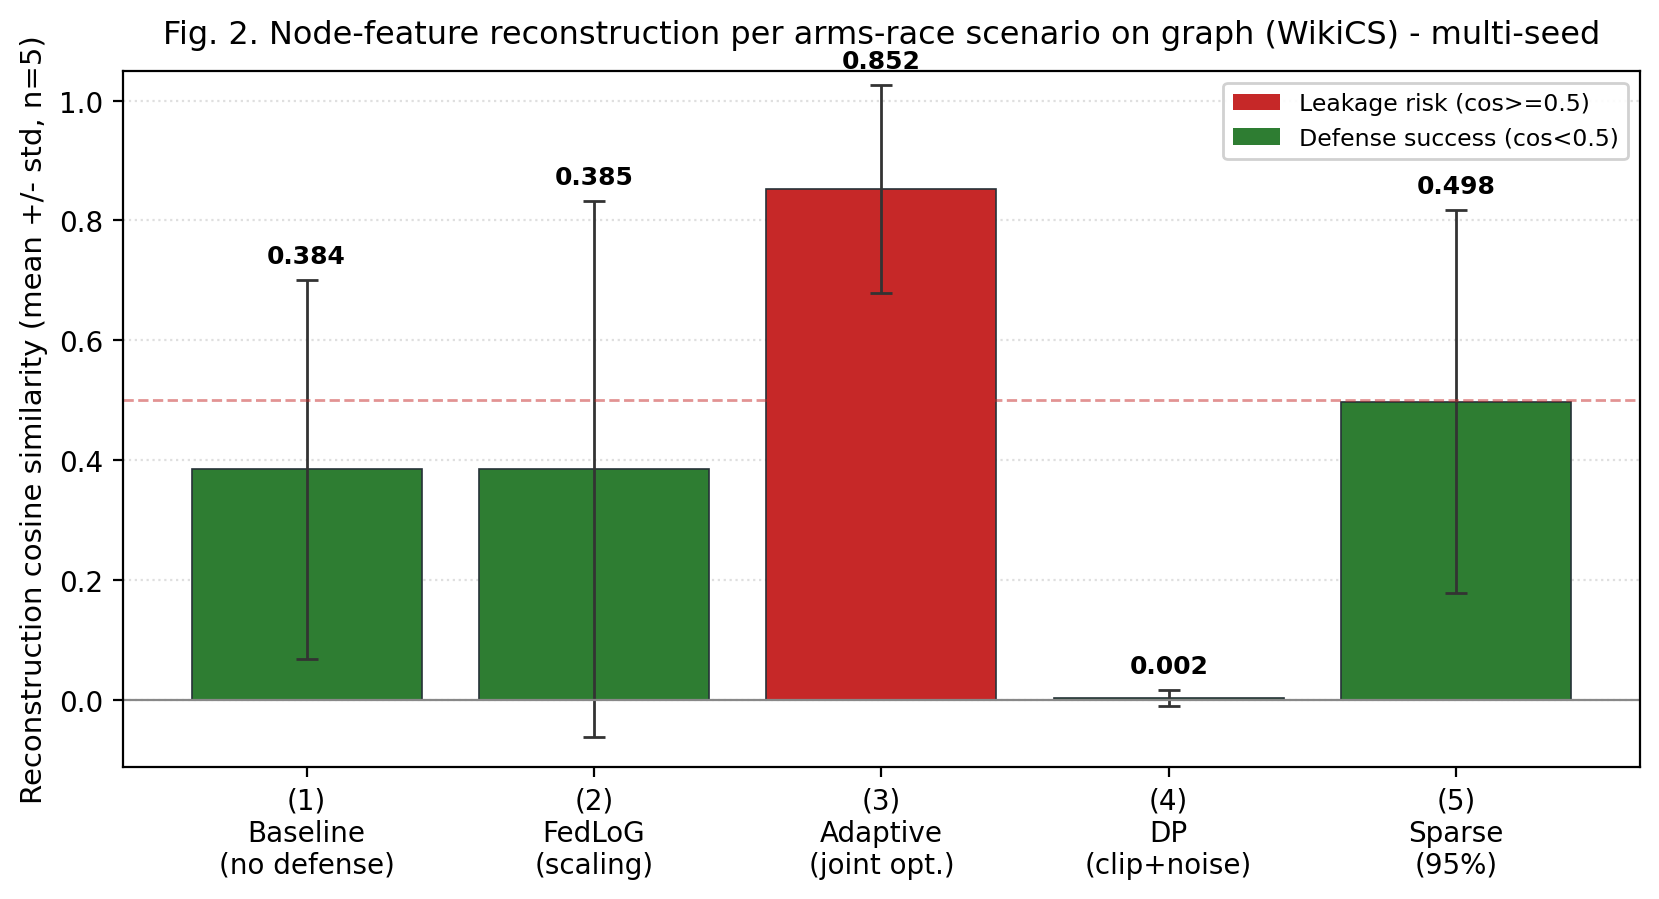
\includegraphics[width=\columnwidth]{fig2_gnn_defense.png}
\caption{Reconstruction cosine per scenario (mean$\pm$std, $n{=}5$). Large error
bars show node-dependent variance; the $\sim$0 for DP shows a consistent
defense.}
\label{fig:gnn_defense}
\end{figure}

\begin{table}[!t]
\caption{Within-Seed Paired Effect --- Net Arms-Race Effect with Variance Removed
($n{=}5$)}
\label{tab:gnn_paired}
\centering
\footnotesize
\begin{tabular}{@{}lccl@{}}
\toprule
\textbf{Transition (same target node)} & \textbf{Mean $\Delta$cos} & \textbf{Sign} & \textbf{Interp.} \\
\midrule
No def. $\to$ scaling & $+0.001\pm0.465$ & mixed & def. void \\
\textbf{Naive $\to$ adaptive} & $\mathbf{+0.467\pm0.414}$ & all $+$ & \textbf{def. broken} \\
\textbf{Adaptive $\to$ DP} & $\mathbf{-0.849\pm0.168}$ & all $-$ & \textbf{strong def.} \\
Adaptive $\to$ sparsify & $-0.354\pm0.223$ & all $-$ & def. (weak) \\
\bottomrule
\end{tabular}
\end{table}

\begin{figure}[!t]
\centering
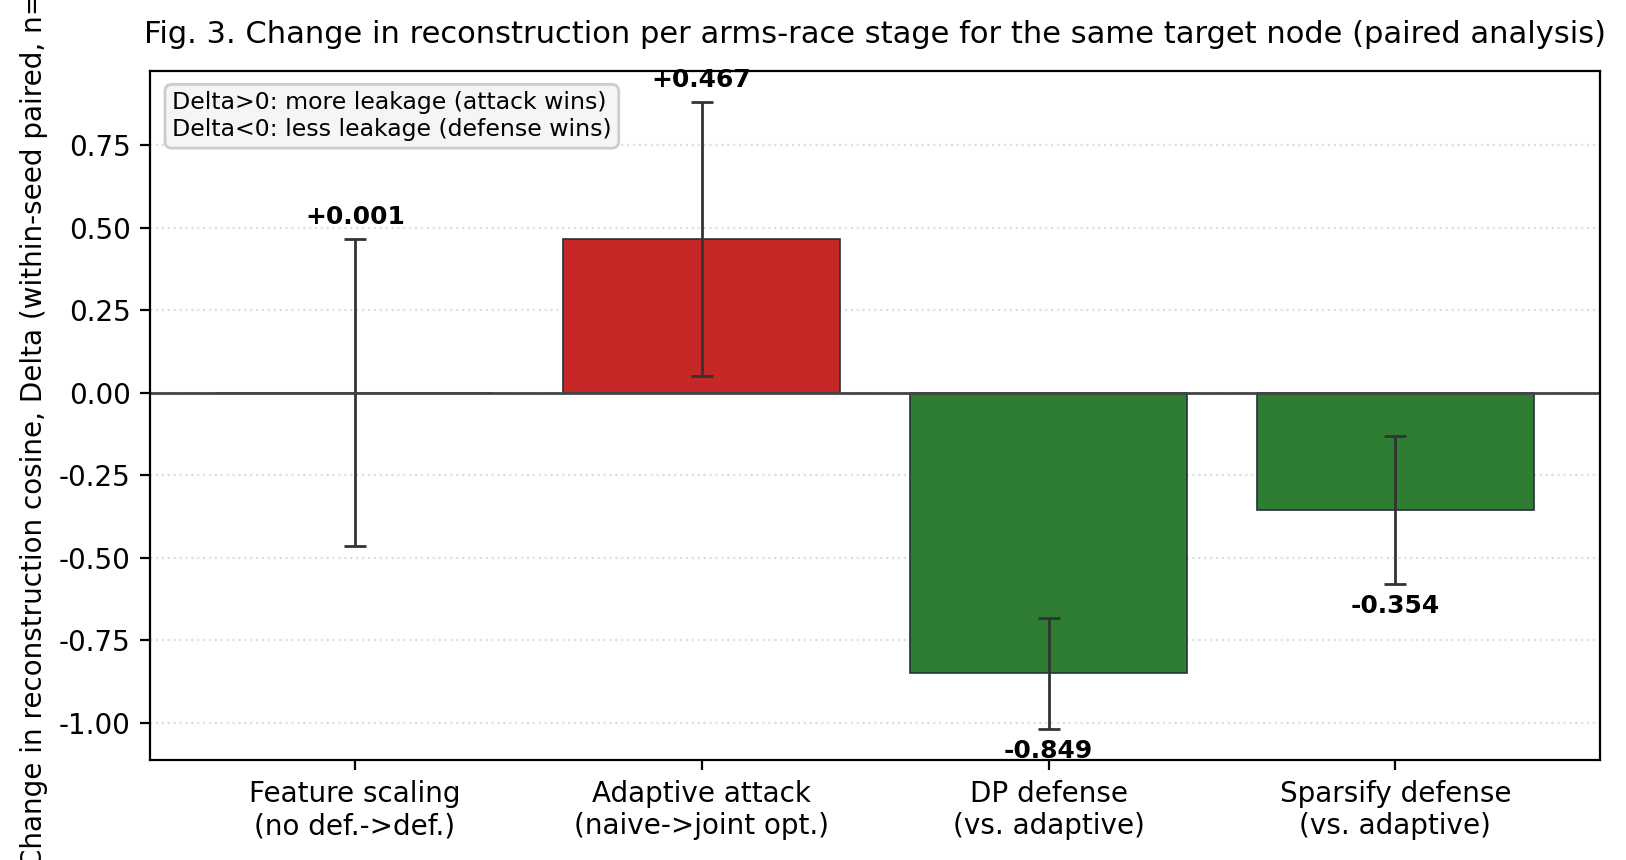
\includegraphics[width=\columnwidth]{fig3_gnn_paired.png}
\caption{Change $\Delta$ in reconstruction per arms-race stage for the same
target node (paired, $n{=}5$). The adaptive attack always raises leakage ($+$);
DP and sparsification always lower it ($-$).}
\label{fig:gnn_paired}
\end{figure}

These results answer RQ3. \textbf{The obfuscation defense (feature scaling) is
unreliable ($\Delta\approx0$) and is consistently nullified by the adaptive
attack ($\Delta\,{+}0.47$, all seeds).} In contrast, \textbf{the
information-destroying defenses (DP, extreme sparsification) consistently lower
the reconstruction quality across all seeds even under the worst case where the
defense mechanism is exposed and combined with the adaptive attack
($\Delta\,{-}0.85, {-}0.35$).} However, their defensive power comes with a utility
cost (DP fidelity 0.001 vs. sparsification 0.702), so the privacy--utility
trade-off must be considered together.

%==============================================================================
\section{Discussion}

\subsection{Summary of Key Findings}
There are four key findings. First (methodological), \textbf{the results of
gradient-leakage experiments have very high variance depending on the target
sample and seed, so single-run ($n{=}1$) reporting is unreliable.} The initial
figures we corrected (image MSE $0.002\to0.0185$; graph cosine $0.9999\to$ a mean
of 0.85, with single runs varying $0.52\sim0.999$) attest to this. Second,
communication-efficiency compression techniques (sparsification, quantization,
pruning) largely fail as defenses, and Soteria sacrifices only utility with no
privacy gain. Third, \textbf{obfuscation (feature scaling) is consistently
nullified by the adaptive attack because of cosine scale invariance.} Fourth,
\textbf{the robustness of a defense comes from ``information destruction,'' not
``secrecy,'' but at the cost of utility.}

\subsection{Comparison of the Image and Graph Domains}
Both domains showed that ``not transmitting the data directly'' does not
guarantee safety, but the manifestations differ. Images are
high-dimensional ($3{\times}32{\times}32$) but have strong spatial correlation
between pixels, so prior knowledge such as TV regularization aids reconstruction;
labels leak 100\% and the reconstruction MSE ($0.0185\pm0.012$) is relatively
stable across samples. In contrast, graph node features are low-dimensional dense
vectors with few structural constraints, exhibiting \textbf{extreme node-dependent
variance} in which some nodes are reconstructed almost perfectly while others are
barely reconstructed at all (cosine $0\sim0.99$). Thus the simple conclusion that
``graphs are uniformly more dangerous than images'' does not hold; the risk
depends heavily on the structural position of the node. This suggests that, when
assessing the privacy risk of relational and tabular data, one must consider not
only the mean but also the variance and the worst case.

\subsection{Obfuscation Defenses vs. Destructive Defenses}
The arms race in Section~V reveals a fundamental principle of defense design. A
defense that merely ``hides'' information, like feature scaling, collapses if the
attacker can also estimate the way it is hidden (the secret variable). This is
the application to FL defense of \textbf{Kerckhoffs's principle}---a system's
security should depend on the secrecy of the key, not of the algorithm. In
contrast, DP noise or extreme sparsification \textbf{irreversibly reduce} the
information content carried by the gradient, so the attacker cannot recover the
lost information even with full knowledge of the defense mechanism. In practice,
therefore, one should adopt destructive defenses as the default---even at the cost
of utility loss---rather than relying on obfuscation.

\subsection{Limitations and Future Work}
We addressed the defects of the initial implementation (unfixed seed,
single-client training, unclipped noise, no utility measurement, $n{=}1$
reporting) in this revision, but the following limitations remain. First,
\textbf{the leakage trend over training progress was inconclusive.} The
reconstruction quality was flat over rounds $0\to20$ (model accuracy $0.12\to0.21$,
i.e., not yet sufficiently trained), and only a single 40-round run was observed
to drop to 0.14. Rigorously confirming the leakage decrease in a sufficiently
converged model is future work. Second, both tracks focused on reconstructing a
batch of size 1 / a single target, and the graph attack assumed the label as
given. Third, DP was corrected to clipping + noise, but a formal privacy
budget ($\varepsilon, \delta$) accounting was not performed (only the strength is
controlled via the noise multiplier). Fourth, the CIFAR-100 model was attacked in
an untrained (worst-case) state due to CPU constraints. Fifth, $n{=}5$ is enough
to reveal the variance but more seeds and targets are desirable for tight
confidence intervals, and the combined effect with secure aggregation and
homomorphic encryption was not addressed. Future work should explore the
privacy--utility curve of DP with $\varepsilon$-accounting, generalization to
diverse GNN architectures, and batch-wise attacks that also reconstruct labels.

%==============================================================================
\section{Conclusion}
This study empirically demonstrated, through reproducible and statistically
rigorous ($n{=}5$) gradient-leakage experiments across the image and graph
domains, that the privacy guarantee of FL does not hold from the mere fact of
``not transmitting raw data.'' At the same time, we emphasize a methodological
lesson: the results of gradient leakage are highly dependent on the sample and
seed, so an impressive single-run figure (e.g., cosine 0.9999) is not
representative. In fact, five repetitions of the same code swung from 0.518 to
0.999, and the risk can be assessed accurately only by considering both the mean
and the variance.

Furthermore, by analyzing the ``vulnerability $\rightarrow$ built-in defense
$\rightarrow$ adaptive attack $\rightarrow$ advanced defense'' arms race via a
within-seed paired comparison with the absolute-value variance removed, we derived
a robust principle. An obfuscation defense such as feature scaling is
consistently nullified (across all seeds) by the adaptive attack because of the
scale invariance of cosine similarity. In contrast, only defenses that
irreversibly destroy information---such as DP with gradient clipping and extreme
sparsification---consistently block leakage even under the worst case where the
defense mechanism is exposed to the adversary. However, such destructive defenses
entail a utility cost as measured by gradient fidelity (DP 0.001 vs.
sparsification 0.702), so the privacy--utility trade-off becomes the key design
variable.

In conclusion, a secure FL system should (1) be designed under a conservative
threat model that assumes the defense is known to the attacker, (2) adopt
defenses that entail information destruction, such as DP, together with a utility
trade-off, and (3) have its effect verified by a multi-seed mean $\pm$ standard
deviation. This is a core lesson for any attempt to apply privacy-preserving
machine learning to real-world services.

%==============================================================================
\begin{thebibliography}{00}

\bibitem{zhu2019dlg}
L. Zhu, Z. Liu, and S. Han, ``Deep Leakage from Gradients,'' in
\textit{Advances in Neural Information Processing Systems (NeurIPS)}, vol.~32,
2019.

\bibitem{zhao2020idlg}
B. Zhao, K. R. Mopuri, and H. Bilen, ``iDLG: Improved Deep Leakage from
Gradients,'' \textit{arXiv preprint arXiv:2001.02610}, 2020.

\bibitem{geiping2020inverting}
J. Geiping, H. Bauermeister, H. Dr\"oge, and M. Moeller, ``Inverting
Gradients --- How Easy Is It to Break Privacy in Federated Learning?,'' in
\textit{Advances in Neural Information Processing Systems (NeurIPS)}, vol.~33,
2020.

\bibitem{mcmahan2017fedavg}
B. McMahan, E. Moore, D. Ramage, S. Hampson, and B. A. y Arcas,
``Communication-Efficient Learning of Deep Networks from Decentralized Data,''
in \textit{Proc. 20th Int. Conf. Artificial Intelligence and Statistics
(AISTATS)}, 2017, pp.~1273--1282.

\bibitem{abadi2016dp}
M. Abadi, A. Chu, I. Goodfellow, H. B. McMahan, I. Mironov, K. Talwar, and
L. Zhang, ``Deep Learning with Differential Privacy,'' in \textit{Proc. 2016
ACM SIGSAC Conf. Computer and Communications Security (CCS)}, 2016,
pp.~308--318.

\bibitem{sun2021soteria}
J. Sun, A. Li, B. Wang, H. Yang, H. Li, and Y. Chen, ``Soteria: Provable
Defense Against Privacy Leakage in Federated Learning From Representation
Perspective,'' in \textit{Proc. IEEE/CVF Conf. Computer Vision and Pattern
Recognition (CVPR)}, 2021, pp.~9311--9319.

\bibitem{hamilton2017sage}
W. L. Hamilton, R. Ying, and J. Leskovec, ``Inductive Representation Learning
on Large Graphs,'' in \textit{Advances in Neural Information Processing Systems
(NeurIPS)}, vol.~30, 2017.

\bibitem{kim2025fedlog}
S. Kim, Y. Lee, Y. Oh, N. Lee, S. Yun, J. Lee, S. Kim, C. Yang, and C. Park,
``Subgraph Federated Learning for Local Generalization,'' in \textit{Int. Conf.
Learning Representations (ICLR)}, 2025, Oral. arXiv:2503.03995.

\bibitem{mernyei2020wikics}
P. Mernyei and C. Cangea, ``Wiki-CS: A Wikipedia-Based Benchmark for Graph
Neural Networks,'' \textit{arXiv preprint arXiv:2007.02901}, 2020.

\bibitem{krizhevsky2009cifar}
A. Krizhevsky, ``Learning Multiple Layers of Features from Tiny Images,''
Technical Report, University of Toronto, 2009.

\end{thebibliography}

\end{document}
